\subsection{Escrevendo HTML das páginas WEB}

As páginas são bem simples. Há uma página \textit{index} e uma página de formulário para passar as credenciais da rede. As páginas e o arquivo de estilização precisam estar numa pasta chamada \textit{data} para serem enviadas ao ESP32.

A página \textit{index} só mostra se o botão selecionado é ON ou OFF. É uma página padrão para o fim do projeto.

\begin{lstlisting}
<div class="content">
  <div class="card-grid">
    <div class="card">
      <p class="card-title"><i class="fas fa-lightbulb"></i> GPIO 2</p>
      <p>
        <a href="on"><button class="button-on">ON</button></a>
        <a href="off"><button class="button-off">OFF</button></a>
      </p>
      <p class="state">State: %STATE%</p>
    </div>
  </div>
</div>
\end{lstlisting}

A página \textit{wifimanager} possui um formulário para passar as credenciais da rede e definir um endereço de acesso ao ESP32 que estará em modo estacionário.

\begin{lstlisting}
<form action="/" method="POST">
  <p>
    <label for="ssid">SSID</label>
    <input type="text" id ="ssid" name="ssid"><br>
    <label for="pass">Password</label>
    <input type="text" id ="pass" name="pass"><br>
    <label for="ip">IP Address</label>
    <input type="text" id ="ip" name="ip" value="192.168.1.200"><br>
    <label for="gateway">Gateway Address</label>
    <input type="text" id ="gateway" name="gateway" value="192.168.1.1"><br>
    <input type ="submit" value ="Submit">
  </p>
</form>
\end{lstlisting}

O código apresentado é apenas uma parte. Para acessá-lo por completo, assim como o arquivo \textit{css} para estilização, acesse os arquivos por esse \href{https://github.com/fabricio-araujo94/microcontroladores/tree/main/wifi_manager_/data}{repositório}.

Para enviar esses arquivos ao ESP32, acessamos a página do PlatformIO, expandimos o menu com o nome da placa com a qual estamos desenvolvendo o projeto (o nosso caso se chama \textit{esp32dev}) e expandimos o menu Platform. Para assim, clicarmos em \textit{Build Filesystem Image}, e quando acabar, clicamos em \textit{Upload Filesystem Image} para enviar os arquivos.

\begin{figure}[H]
    \centering
    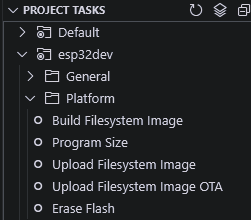
\includegraphics[width=0.5\linewidth]{img/build_image.png}
    \caption{Criando imagem.}
    \label{fig:build-image}
\end{figure}